% Options for packages loaded elsewhere
\PassOptionsToPackage{unicode}{hyperref}
\PassOptionsToPackage{hyphens}{url}
%
\documentclass[
]{article}
\usepackage{amsmath,amssymb}
\usepackage{lmodern}
\usepackage{iftex}
\ifPDFTeX
  \usepackage[T1]{fontenc}
  \usepackage[utf8]{inputenc}
  \usepackage{textcomp} % provide euro and other symbols
\else % if luatex or xetex
  \usepackage{unicode-math}
  \defaultfontfeatures{Scale=MatchLowercase}
  \defaultfontfeatures[\rmfamily]{Ligatures=TeX,Scale=1}
\fi
% Use upquote if available, for straight quotes in verbatim environments
\IfFileExists{upquote.sty}{\usepackage{upquote}}{}
\IfFileExists{microtype.sty}{% use microtype if available
  \usepackage[]{microtype}
  \UseMicrotypeSet[protrusion]{basicmath} % disable protrusion for tt fonts
}{}
\makeatletter
\@ifundefined{KOMAClassName}{% if non-KOMA class
  \IfFileExists{parskip.sty}{%
    \usepackage{parskip}
  }{% else
    \setlength{\parindent}{0pt}
    \setlength{\parskip}{6pt plus 2pt minus 1pt}}
}{% if KOMA class
  \KOMAoptions{parskip=half}}
\makeatother
\usepackage{xcolor}
\usepackage[margin=1in]{geometry}
\usepackage{graphicx}
\makeatletter
\def\maxwidth{\ifdim\Gin@nat@width>\linewidth\linewidth\else\Gin@nat@width\fi}
\def\maxheight{\ifdim\Gin@nat@height>\textheight\textheight\else\Gin@nat@height\fi}
\makeatother
% Scale images if necessary, so that they will not overflow the page
% margins by default, and it is still possible to overwrite the defaults
% using explicit options in \includegraphics[width, height, ...]{}
\setkeys{Gin}{width=\maxwidth,height=\maxheight,keepaspectratio}
% Set default figure placement to htbp
\makeatletter
\def\fps@figure{htbp}
\makeatother
\setlength{\emergencystretch}{3em} % prevent overfull lines
\providecommand{\tightlist}{%
  \setlength{\itemsep}{0pt}\setlength{\parskip}{0pt}}
\setcounter{secnumdepth}{-\maxdimen} % remove section numbering
\ifLuaTeX
  \usepackage{selnolig}  % disable illegal ligatures
\fi
\IfFileExists{bookmark.sty}{\usepackage{bookmark}}{\usepackage{hyperref}}
\IfFileExists{xurl.sty}{\usepackage{xurl}}{} % add URL line breaks if available
\urlstyle{same} % disable monospaced font for URLs
\hypersetup{
  pdftitle={A Predictive Model for ODI World Cup Matches},
  pdfauthor={Krishna Kumar, Srihari Srinivasan},
  hidelinks,
  pdfcreator={LaTeX via pandoc}}

\title{A Predictive Model for ODI World Cup Matches}
\author{Krishna Kumar, Srihari Srinivasan}
\date{APR 30, 2023}

\begin{document}
\maketitle

\hypertarget{introduction}{%
\subsection{Introduction}\label{introduction}}

Given that this is a One Day International (ODI) World Cup year, our
analysis of batting and bowling performance metrics on the margin of
victory, \texttt{mov}, is focused on prior World Cup matches. With
knowledge of how the ODI format has changed since the introduction of
the shorter, Twenty20 (T20) format, particularly the 2007 T20 World Cup,
we have limited our data to the last five ODI World Cups (2003, 2007,
2011, 2015, and 2019). After wrangling six batting metrics and four
bowling metrics from 4774 individual player performances, we are looking
to build a predictive model and gain insight as to which metrics, if
any, have an effect on \texttt{mov}. In doing so, while this may be
beyond the scope of this project, we hope to ultimately use our model to
predict the outcome of the 2023 ODI World Cup.

\hypertarget{exploratory-analysis}{%
\subsection{Exploratory Analysis}\label{exploratory-analysis}}

\hypertarget{response-variable}{%
\subsubsection{Response Variable}\label{response-variable}}

\texttt{mov} is the difference between the target set by the team
batting first and the total that the chasing team achieved. For example,
in a 2003 match between England and Pakistan, England scored 246 runs,
setting 247 as the target for Pakistan to chase. They, however, were
bowled out for 134, resulting in England winning by 112 runs. Therefore,
the \texttt{mov} for this match is calculated as
\(winner\_margin / target = 112 / 247 = 0.453\).\\

The figure below is a boxplot of \texttt{mov} values.\\

\includegraphics[width=0.6\linewidth]{Kumar-Srinivasan-Project2_files/figure-latex/unnamed-chunk-2-1}

\begin{verbatim}
##    Min. 1st Qu.  Median    Mean 3rd Qu.    Max. 
## -0.8400 -0.1300  0.0570  0.0709  0.3390  0.9010
\end{verbatim}

From the figure and summary, we can see that \texttt{mov} is
approximately normally distributed on 7.1\%. The single outlier is a
2011 match between Kenya and New Zealand in which Kenya lost by 84.0\%.
While large \texttt{mov} values can be attributed to a blowout, the
extreme values probably occurred due to a wide skill gap between two
teams. New Zealand, for example, is an established cricketing nation
with a strong, experienced team compared to Kenya.

\hypertarget{predictor-variables}{%
\subsubsection{Predictor Variables}\label{predictor-variables}}

Batting metrics:\\
Given that top-order batsmen (players 1, 2, and 3) generally play a
different role to that of middle-order batsmen (players 4, 5, 6, and 7),
these metrics have been separated by batting position.\\
1. \texttt{to\_runs\_pct} - percentage of total runs scored by the
top-order\\
2. \texttt{mo\_runs\_pct} - percentage of total runs scored by the
middle-order\\
3. \texttt{to\_mins\_pct} - percentage of total time spent in crease by
the top-order\\
4. \texttt{mo\_mins\_pct} - percentage of total time spent in crease by
the middle-order\\
5. \texttt{to\_bf\_pct} - percentage of total balls faced by the
top-order\\
6. \texttt{mo\_bf\_pct} - percentage of total balls faced by the
middle-order\\
7. \texttt{pct\_4s} - percentage of total runs that are 4s\\
8. \texttt{pct\_6s} - percentage of total runs that are 6s\\
9. \texttt{to\_sr} - average strike rate of the top-order\\
10. \texttt{mo\_sr} - average strike rate of the middle-order\\

Bowling metrics:\\
1. \texttt{bowlers\_used} - total number of bowlers used\\
2. \texttt{pct\_mdns} - percentage of total overs that are maidens (an
over in which no runs are scored)\\
3. \texttt{wkts} - total number of wickets taken\\
4. \texttt{econ} - average number of runs conceded per over bowled\\

The figures below are scatterplots of the pairwise relationship between
predictor variables.\\

\includegraphics[width=1\linewidth]{Kumar-Srinivasan-Project2_files/figure-latex/unnamed-chunk-3-1}

\includegraphics[width=1\linewidth]{Kumar-Srinivasan-Project2_files/figure-latex/unnamed-chunk-4-1}

\includegraphics[width=1\linewidth]{Kumar-Srinivasan-Project2_files/figure-latex/unnamed-chunk-5-1}

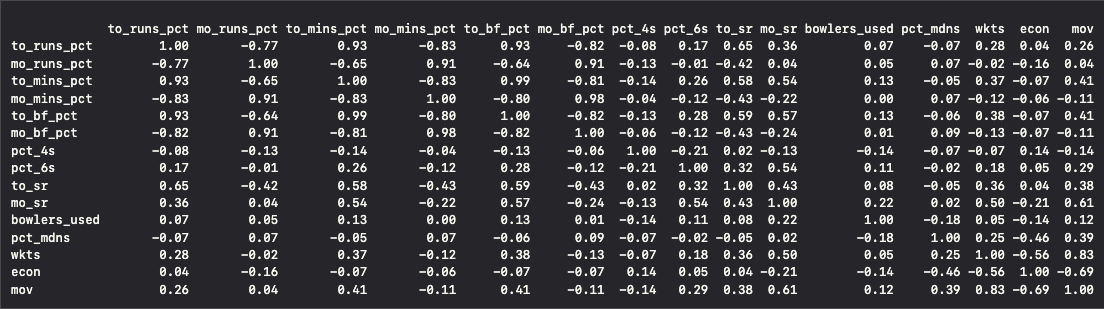
\includegraphics[width=1\linewidth]{cor}

From the figures and correlation matrix, we can see that
\texttt{runs\_pct}, \texttt{mins\_pct}, and \texttt{bf\_pct} have high
collinearity. This exists because the impact of a top-order batsman is
not entirely independent of a middle-order batsman. Although the
correlation of certain variables exceeds \(\pm 0.80\), we decided to let
the backward step-wise process filter out and select the metrics with
the greatest effect on \texttt{mov}.

\hypertarget{model-development}{%
\subsection{Model Development}\label{model-development}}

Our objective at each step of the backward step-wise selection process
is to minimize \emph{RMSE} and maximize \emph{adjusted R-squared}.
First, we split our data into training and test sets. The training set
consists of World Cup matches from 2003 to 2015, whereas the test set is
composed solely of 2019 data.\\

\begin{verbatim}
## 
## Call:
## lm(formula = mov ~ ., data = train_set)
## 
## Residuals:
##      Min       1Q   Median       3Q      Max 
## -0.31506 -0.08535  0.00520  0.08190  0.33314 
## 
## Coefficients:
##                Estimate Std. Error t value Pr(>|t|)    
## (Intercept)  -0.4882452  0.1587330  -3.076 0.002467 ** 
## to_runs_pct  -0.8628535  0.2637747  -3.271 0.001310 ** 
## mo_runs_pct  -0.8042278  0.2725020  -2.951 0.003638 ** 
## to_mins_pct   0.6292071  0.6287787   1.001 0.318482    
## mo_mins_pct   0.0862708  0.6099045   0.141 0.887692    
## to_bf_pct     0.6309025  0.6772988   0.931 0.352991    
## mo_bf_pct     1.1391437  0.6397287   1.781 0.076853 .  
## pct_4s        0.0158615  0.1478799   0.107 0.914717    
## pct_6s        0.2999686  0.1898668   1.580 0.116095    
## to_sr         0.0023055  0.0006801   3.390 0.000880 ***
## mo_sr         0.0020120  0.0005138   3.916 0.000133 ***
## bowlers_used -0.0208609  0.0112526  -1.854 0.065587 .  
## pct_mdns      0.6888521  0.1977250   3.484 0.000637 ***
## wkts          0.0451133  0.0046679   9.665  < 2e-16 ***
## econ         -0.0713556  0.0086423  -8.257 5.15e-14 ***
## ---
## Signif. codes:  0 '***' 0.001 '**' 0.01 '*' 0.05 '.' 0.1 ' ' 1
## 
## Residual standard error: 0.132 on 161 degrees of freedom
## Multiple R-squared:  0.8906, Adjusted R-squared:  0.881 
## F-statistic: 93.57 on 14 and 161 DF,  p-value: < 2.2e-16
\end{verbatim}

After training our model using all 14 predictor variables, we observe an
\emph{adjusted R-squared} value of 0.881, meaning we are able to explain
88.1\% of the variation in \texttt{mov} with all 14 variables.

Using this model, we predict \texttt{mov} based on the test set and
calculate the \emph{RMSE} value displayed below.

\begin{verbatim}
## [1] 0.1531916
\end{verbatim}

Normalizing this by dividing \emph{RMSE} by the range of \texttt{mov}
from the test set results in the following value.

\begin{verbatim}
## [1] 0.1327484
\end{verbatim}

We further verify these relationships with the use of added-variable
plots.\\

\includegraphics[width=1\linewidth]{Kumar-Srinivasan-Project2_files/figure-latex/unnamed-chunk-10-1}

Backward step-wise selection removes each of these 14 variables from the
model, one at a time, and checks for improvement in the performance
metric \emph{RMSE}. Using a loop, we remove one variable at a time from
the training set. We remove the \(i\)-th column using
\texttt{train\_set{[},-i{]}}. This allows us to iterate through columns
1 to 14.

We want to find the lowest \emph{RMSE} value from the table below and
remove the predictor variable associated with it. The lowest value
appears to be 0.142 which is the 10th row and corresponds to the
\texttt{mo\_sr} variable. We will then remove this variable from the
training set and repeat this process.

\begin{verbatim}
##         vals
## 1  0.1541412
## 2  0.1452954
## 3  0.1559078
## 4  0.1532753
## 5  0.1513644
## 6  0.1504844
## 7  0.1534606
## 8  0.1549225
## 9  0.1627135
## 10 0.1423925
## 11 0.1457553
## 12 0.1601905
## 13 0.1797444
## 14 0.1889362
\end{verbatim}

The table below shows all of the \emph{RMSE} values after removing
\texttt{mo\_sr}. The lowest value appears to be 0.138 which is the 10th
row and corresponds to the \texttt{bowlers\_used} variable. We will then
remove this variable from the training set and repeat this process.

\begin{verbatim}
##         vals
## 1  0.1401743
## 2  0.1407669
## 3  0.1453592
## 4  0.1425708
## 5  0.1396741
## 6  0.1411606
## 7  0.1442560
## 8  0.1410817
## 9  0.1454950
## 10 0.1382726
## 11 0.1493844
## 12 0.1793459
## 13 0.1749365
\end{verbatim}

The table below shows all of the \emph{RMSE} values after removing
\texttt{bowlers\_used}. The lowest value appears to be 0.136 which is
the 5th row and corresponds to the \texttt{to\_bf\_pct} variable. We
will then remove this variable from the training set and repeat this
process.

\begin{verbatim}
##         vals
## 1  0.1373298
## 2  0.1373746
## 3  0.1410767
## 4  0.1384229
## 5  0.1362954
## 6  0.1376920
## 7  0.1401080
## 8  0.1379419
## 9  0.1431505
## 10 0.1426865
## 11 0.1698732
## 12 0.1778158
\end{verbatim}

The table below shows all of the \emph{RMSE} values after removing
\texttt{to\_bf\_pct}. The lowest value appears to be 0.1339 which is the
7th row and corresponds to the \texttt{pct\_6s} variable. We will then
remove this variable from the training set and repeat this process.

\begin{verbatim}
##         vals
## 1  0.1389401
## 2  0.1362618
## 3  0.1409512
## 4  0.1340669
## 5  0.1368344
## 6  0.1380571
## 7  0.1338812
## 8  0.1422163
## 9  0.1401365
## 10 0.1693369
## 11 0.1755852
\end{verbatim}

The table below shows all of the \emph{RMSE} values after removing
\texttt{pct\_6s}. The lowest value appears to be 0.12886 which is the
4th row and corresponds to the \texttt{mo\_mins\_pct} variable. We will
then remove this variable from the training set and repeat this process.

\begin{verbatim}
##         vals
## 1  0.1383374
## 2  0.1329154
## 3  0.1391656
## 4  0.1288591
## 5  0.1336530
## 6  0.1343008
## 7  0.1402499
## 8  0.1408747
## 9  0.1623683
## 10 0.1697544
\end{verbatim}

The table below shows all of the \emph{RMSE} values after removing
\texttt{mo\_mins\_pct}. The lowest value appears to be 0.1289 which is
the 2nd row and corresponds to the \texttt{mo\_runs\_pct} variable.
However, since this value is slightly higher than the previous lowest
\emph{RMSE} value, we can stop the process and create our final model.

\begin{verbatim}
##        vals
## 1 0.1355545
## 2 0.1288692
## 3 0.1416369
## 4 0.1300969
## 5 0.1294081
## 6 0.1321559
## 7 0.1363999
## 8 0.1687512
## 9 0.1639578
\end{verbatim}

Our final model, after taking out \texttt{mo\_sr},
\texttt{bowlers\_used}, \texttt{to\_bf\_pct}, \texttt{pct\_6s}, and
\texttt{mo\_mins\_pct}, has an \emph{adjusted R-Squared} of 0.857 and a
\emph{RMSE} value of 0.129. Therefore, we are able to account for 85.7\%
of the variation in \texttt{mov}.

\begin{verbatim}
## 
## Call:
## lm(formula = mov ~ ., data = train_min5)
## 
## Residuals:
##      Min       1Q   Median       3Q      Max 
## -0.30963 -0.10122 -0.00361  0.08405  0.39258 
## 
## Coefficients:
##               Estimate Std. Error t value Pr(>|t|)    
## (Intercept) -0.6843105  0.1395203  -4.905 2.22e-06 ***
## to_runs_pct -0.8401548  0.2325325  -3.613 0.000401 ***
## mo_runs_pct -0.0201497  0.2208547  -0.091 0.927416    
## to_mins_pct  1.3362872  0.2441730   5.473 1.61e-07 ***
## mo_bf_pct    0.4915536  0.2690876   1.827 0.069535 .  
## pct_4s       0.0394186  0.1546612   0.255 0.799138    
## to_sr        0.0037793  0.0006734   5.612 8.23e-08 ***
## pct_mdns     0.7987057  0.2083292   3.834 0.000179 ***
## wkts         0.0512169  0.0049609  10.324  < 2e-16 ***
## econ        -0.0654071  0.0090644  -7.216 1.82e-11 ***
## ---
## Signif. codes:  0 '***' 0.001 '**' 0.01 '*' 0.05 '.' 0.1 ' ' 1
## 
## Residual standard error: 0.1448 on 166 degrees of freedom
## Multiple R-squared:  0.8642, Adjusted R-squared:  0.8569 
## F-statistic: 117.4 on 9 and 166 DF,  p-value: < 2.2e-16
\end{verbatim}

Normalizing the \emph{RMSE} results in the below value.

\begin{verbatim}
## [1] 0.0740144
\end{verbatim}

Verifying the relationships with the updated added-variable plots.\\

\includegraphics[width=1\linewidth]{Kumar-Srinivasan-Project2_files/figure-latex/unnamed-chunk-19-1}

\hypertarget{model-analysis}{%
\subsection{Model Analysis}\label{model-analysis}}

\[
\text{mov} = -0.684 + -0.84*\text{to_runs_pct}
\]

To analyze our final model, we test it on the entire dataset of all five
World Cups. The model's final \emph{adjusted R-squared} is 0.857, which
means we are able to account for 85.7\% of the variation in
\texttt{mov}. With a final \emph{RMSE} of 0.138, our predicted values
generally differ from the observed values of \texttt{mov} by 13.8\%.
However, normalizing this value results in 0.08 or 8\%. Before applying
the backwards step-wise process, our first model had an \emph{adjusted
R-squared} of 0.881 and a \emph{RMSE} of 0.153. Comparing the two
models, our \emph{adjusted R-squared} decreased by around 3\%, however
we were also able to decrease \emph{RMSE} by around 2\%. We believe that
this trade-off is ultimately worth it as this model best minimizes the
difference between predicted and observed values. Thereby, prioritizing
the accuracy of the model's predictions rather than the overall quality
of the model's fit to the data.

We can analyze our model's accuracy by testing it using one random ODI
World Cup match throughout the years. The match we used is a match from
the 2007 ODI World Cup of Bangladesh versus New Zealand. The
\texttt{mov} for the match was -0.413 and the predicted \texttt{mov} was
-0.619. Our predicted \texttt{mov} value is -0.206 off of the observed
\texttt{mov} value which indicates our model is fairly accurate and not
too far off of the observed value.

\begin{verbatim}
## [1] -0.413
\end{verbatim}

\begin{verbatim}
##         68 
## -0.6192819
\end{verbatim}

\begin{verbatim}
##         68 
## -0.2062819
\end{verbatim}

The figure below is a scatterplot of the predicted values and their
residuals.\\

\includegraphics[width=0.6\linewidth]{Kumar-Srinivasan-Project2_files/figure-latex/unnamed-chunk-22-1}

\hypertarget{conclusion}{%
\subsection{Conclusion}\label{conclusion}}

We can conclude that \texttt{to\_runs\_pct}, \texttt{mo\_runs\_pct},
\texttt{to\_mins\_pct}, \texttt{mo\_bf\_pct}, \texttt{pct\_4s},
\texttt{to\_sr}, \texttt{pct\_mdns}, \texttt{wkts}, and \texttt{econ}
are the variables that best predict \texttt{mov}. Due to either
multicollinearity or low correlation, \texttt{mo\_mins\_pct},
\texttt{to\_bf\_pct}, \texttt{pct\_6s}, \texttt{mo\_sr}, and
\texttt{bowlers\_used} were excluded from our model. This is somewhat
surprising as we believed that \texttt{mo\_mins\_pct} and
\texttt{mo\_sr} would have a greater impact on \texttt{mov},
particularly since the role of middle-order batsmen has been heightened
since the introduction of the T20 format. The lack of \texttt{pct\_6s}
inclusion in the model is not as surprising as we expect batsmen to
score more of their boundaries through 4s in a longer format where each
wicket is more ``valuable.'' We initially included
\texttt{bowlers\_used} on a suspicion that the more bowlers a team
employed, the less faith they had in their front-line bowlers, implying
that they had a weaker bowling lineup overall. This, however, was proven
not to be the case as whether a team used 4 bowlers or 8, there was no
effect on \texttt{mov}. Given more time, we would incorporate non-World
Cup data in order to better assess whether

\end{document}
